% Chapter Template

\chapter{Introduction} % Main chapter title

\label{Introduction} % Change X to a consecutive number; for referencing
% this chapter elsewhere, use \ref{ChapterX}
%Default was: Chapter 1 .\emph{Introduction} 
\lhead{\emph{Introduction}} % Change X to a consecutive number;
% this is for the header on each page - perhaps a shortened title

%----------------------------------------------------------------------------------------
%	SECTION 1
%----------------------------------------------------------------------------------------


    
    

\section{Soft matter and biopolymers}
Soft matter, also known as complex fluids, is a subfield of condensed
matter, comprising systems which:
\begin{enumerate*}[label=\bfseries\alph*)]
 
\item organize at many different length scales, into
many different forms and it classifies as something in between the
ordered solids and disordered liquids.\
\item its conformation is heavily
influenced by thermal fluctuations in the energy scale comparable to the room
temperature. This characteristic allows conformational changes where complex
behaviour can occur, life as the outermost example.
\end{enumerate*}

Soft matter includes liquids, colloids, polymers, foams, gels, granular
materials, surfactants, liquids crystals and some biological materials.
Pierre-Gilles de Gennes, who has been called the ``founding father of soft
mater'' received the Nobel Prize in physics in $1991$ ``for discovering that 
methods developed for studying order phenomena in simple systems can be 
generalized to more complex forms of matter, in particular to liquid  crystals
and polymers''\citep{de_gennes_pierre-gilles_????}
 
The biological soft materials spam as well different length scales. From sugar
chains structures to active gels inside cells. In the
lowest scale, we find the biopolymers, which are classified as polysaccharides
(cellulose, pectin),  polynucleotides (RNA, DNA) or polypeptides (proteins).
 
Most of biopolymers are considered semi-flexible. Something in between
rigid rods and completely flexible (loose) chains.  To formalize this
distinction we need to introduce $2$ parameters that characterize a polymer
chain: the \emph{persitence length} \gls{Lp} which is the typical length scale
for the decay of tangent-tanget correlations, and the \emph{countour length}
\gls{Lc}, which is defined as the maximum end-to-end distance of a linear
polymer chain.

A chain is considered flexible when $\ell_p<<L_c$, and rigid when the opposite
holds. Completely flexible chains exhibit a purely entropic elastic
response, and rigid filaments display no entropic, but purely enthalpic
response. Semi-flexible biopolymers have a similar magnitude of $\ell_p$ and
$L_c$. These kind of filaments does not form loops or knots, but they are
flexible enough to have thermal bending
fluctuations\citep{storm_nonlinear_2005}. They behave like rods scales smaller
than $\ell_p$ and like random coils in larger scales where the entropic behavior
dominates.

\section{Semiflexible single chains: WLC model}
Single semiflexible chains can be modeled with great success with the
\emph{worm-like chain} (WLC) also known as \emph{Kratky-Porod} model.
\citep{rubinstein_polymer_2003, schuster_hierarchical_2011}. This model has
became a standard in the field thanks to the agreement with experiments in low
and large scales.
But it is not completely satisfactory in middle scales, where occurs the
crossover between enthalpic and entropic behavior.\citet{hsu_breakdown_2011}

$$H_{bend}=\frac{\kappa}{2} \int ds|\frac{\partial \textbf{t}}{\partial s}|$$

where $k\equiv\kbend{}$ is the bending modulus, \textbf{t} is a unit tangent
vector along the chain and $s$ is the coordinate of the position along the
backbone. In the WLC model we can relate the persistance length with the bending
modulus via: $\lp{}=2\kbend{}/((d-1)\kbolt{}T)$ where $d$ is the space
dimensionality.

For nearly straight filaments $\frac{\partial \textbf{t}}{\partial s}$ can be
expressed via the transverse deviation $u(x)$ of the chain from its straight
conformation. $\frac{\partial \textbf{t}}{\partial s}=u''(x)$. If the chain is
under a tensional force from one end (and the other end fixed), we can add the
term $-fL$ to the Hamiltonian, where L being the end to end distance. The
Hamiltonian with this force $f_B$ in transverse coordinates :
\begin{equation}\label{WLC_H}
H=\frac{1}{2}\int_0^{L_c} dx\Big[\kappa|u''|^2 + f_B|u'|^2\Big]
\end{equation}

where $L_c$ is the contour length of the chain.
The applicability of\ref{WLC_H} must be questioned in some cases since it
neglects excluded volume (steric repulsion effects) between the
chain constituents completely.\citet{hsu_breakdown_2011}. For very stiff polymer
these excluded volume considerations could be safely ignored.

Such a chain can respond to transverse and also to longitudinal forces by either
bending or stretching/compressing. We can explore further the force-extension
(FE) relationship, decomposing u in Fourier series:
\begin{equation}\label{WLC_ufourier}
u(x)=\sum_q u_q \sin(qx)
\end{equation}
with the wave vector $q=n\pi/L_c$. We can rewrite \ref{WLC_H} as:
\begin{equation}\label{WLC_Hq}
H=\frac{1}{2}\int_0^{L_c} dx\Big[\kappa|u''|^2 + f_B|u'|^2\Big] =
\frac{L_c}{4}\sum_q (\kappa q^4 + f_Bq^2)u_q^2
\end{equation}

To calculate the equilibrium amplitude we shall use the equipartition theorem:
\begin{equation}\label{equipartition}
\Big\langle x_m\frac{\partial H}{\partial x_n} \Big\rangle= \delta_{mn}\kbolt{}T
\end{equation}

where H is the Hamiltonian or energy function and $x_n$ corresponds to the
% degrees of freedom in the phase space. Note than the system must be ergodic and in
thermal equilibrium to apply the equipartition theorem. A system is ergodic when
the ensemble average (mean over all the possible states) is equal to the time average (mean over all time
steps). Also the equipartition theorem does not hold when the
thermal energy $\kbolt{}T$ is smaller than the quantum energy spacing for a
particular degree of freedom because the breakage of the energy continuum. This
strong requirement does not hold for many soft matter systems. The idea behind
the equipartition theorem is that the energy in thermal equilibrium is shared
equally among all its components.

Applying \ref{equipartition}to \ref{WLC_Hq}, the equilibrium amplitudes
$u_q^{eq} $ satisfy:
\begin{equation}\label{equipartition_uq}
\langle u_q^{eq}\rangle=\frac{2\kbolt{}T}{L_c(\kappa{}q^4+f_Bq^2)}
\end{equation}
We can now calculate $\delta L$, the difference between the filament's contour
length and the equilibrium length.
\begin{equation}\label{deltaL}
\Delta L= \int dx \Big[ \sqrt{1+|\partial u/\partial x|^2} -1\Big]\simeq
\frac{1}{2} \int dx |\partial u/\partial x|^2 = L_c \sum_q q^2 u_q^2
\end{equation}

Using \ref{equipartition_uq} and including a factor of $2$ due to both
degrees of freedom of the transverse displacements from the straight
conformation:
\begin{equation}\label{deltaLmean}
\langle\Delta L\rangle = \kbolt{}T\sum_q \frac{1}{\kappa{}q^2+f_B}
\end{equation}

The result is most convenient expressed un terms of scaled difference between
the extension at force $f_B$ and that at zero force\citep{storm_nonlinear_2005}:
\begin{equation}\label{WLCdisplacement}
\delta l=\langle\Delta L\rangle_{f=0} - \langle\Delta L\rangle_{f_B} =
\frac{L_c^2}{\ell_p\pi^2} \sum_q \frac{\varphi}{n^2(n^2 + \varphi)}
\end{equation} 
where $\varphi = f_BL_c^2/\kappa{}\pi^2$

\ref{WLCdisplacement} can be inverted to yield a force-extension (FE)
relation:\citep{marko_stretching_1995}:
\begin{equation}\label{FEMarko}
f(x)=\frac{\kbolt{}T}{\ell_p} \Big[ \frac{1}{4(1 - x/L_c)^2} 
-\frac{1}{4}+\frac{x}{L_c} \Big]
\end{equation}

which diverges as $f \sim (x - L_c)^{-2}$ as $x\rightarrow L_c$
%TODO: ADD INFO ABOUT FE

This force-extension curve is of central importance in this project. This FE can
be measured using optical tweezers, experimental technique available in our
group. Optical tweezers are able to trap and manipulate beads of
nanometric size with high
precision\citep{svoboda_direct_1993,svoboda_biological_1994}.
Biopolymer chains can be attached to these beads using linkage molecules, and then study the force-extension of the
chain when the force is applied by the movement of the trap in the tweezers, and
the extension is measured tracking the beads under the microscopy.

\begin{figure}[h]

\begin{minipage}{0.65\textwidth}
\subfloat[]{%
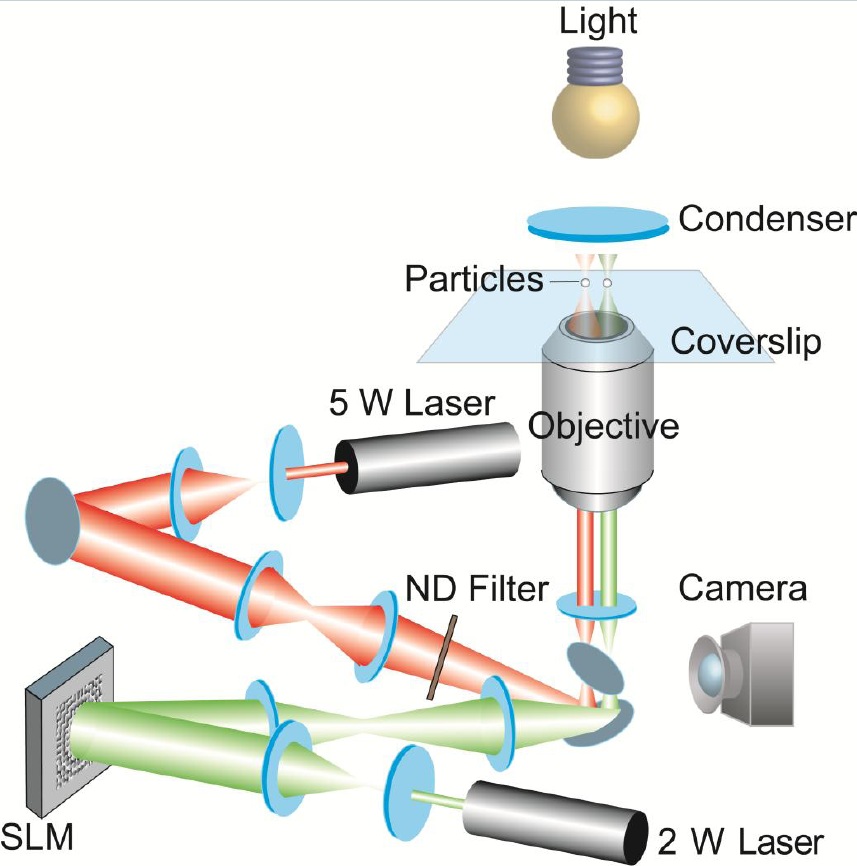
\includegraphics[width=0.9\textwidth]{Figures/tweezers_configuration.png}%
\label{tweezers-configuration}}
\end{minipage}
\begin{minipage}{0.35\textwidth}
% \begin{minipage}{0.5\textwidth}
\subfloat[]{%
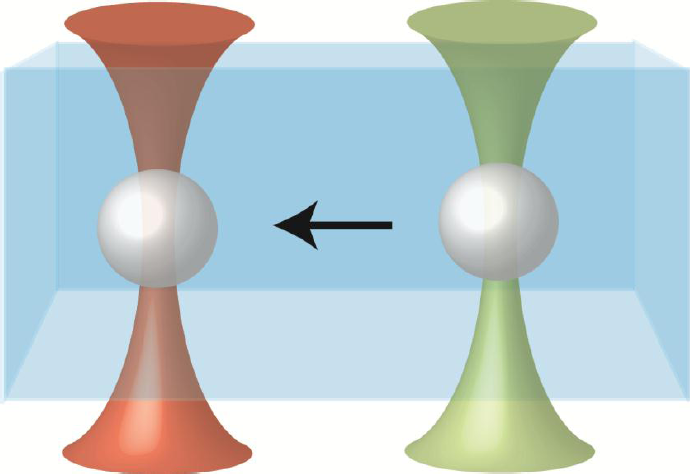
\includegraphics[width=0.9\textwidth]{Figures/tweezers_particles.png}%
\label{tweezers-particles}}

\subfloat[]{%
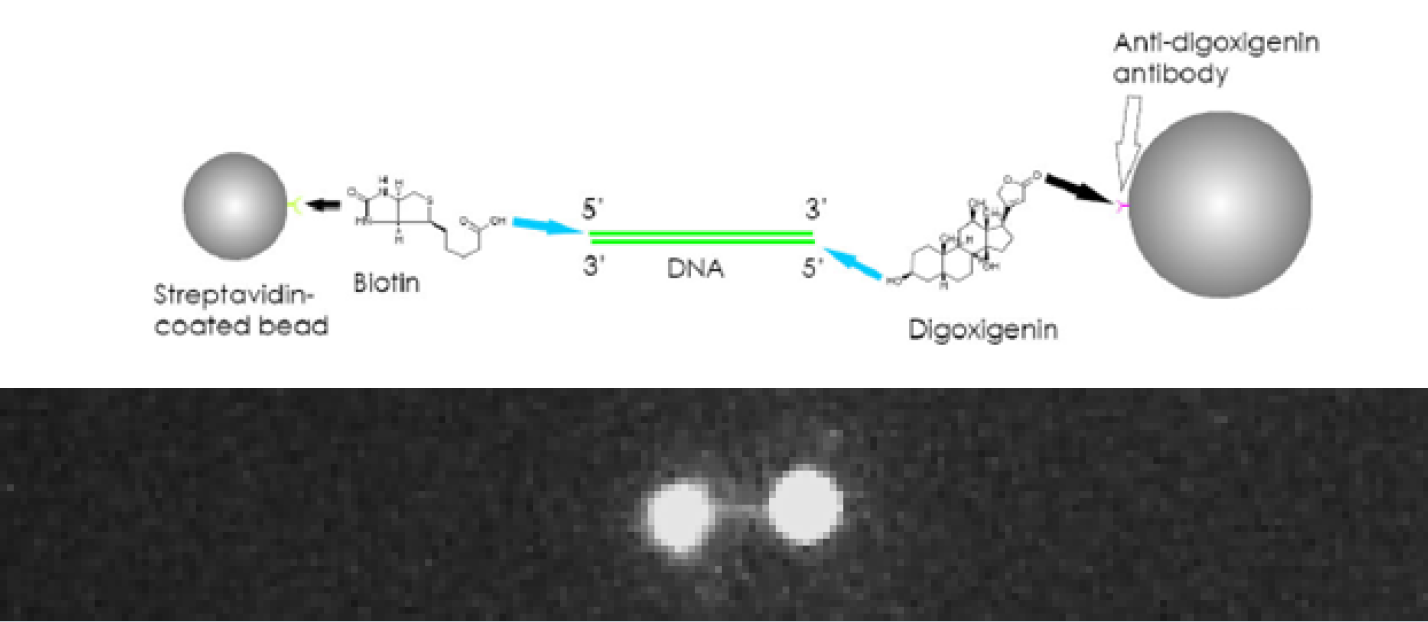
\includegraphics[width=0.9\textwidth,height=3cm]{Figures/tweezers_linkage.png}%
\label{tweezers-linkage}}
\end{minipage}



\caption[Optical Tweezers]{\subref{tweezers-configuration} Current
optical tweezers configuration in our lab. \subref{tweezers-particles}
Exertion of force moving the right trap. One of the bead (red-left) is fixed by
the most powerful trap. \subref{tweezers-linkage} Linkage of the
 polymer stained with fluorescence particles (double stranded DNA) to the beads,
 and below, visualization of the fluorescence. Images by courtesy of group mate,
 Sandy Sue. }
\label{fig:optical_tweezers}
\end{figure}

%  Since the bending rigidity of the polymer is
% of the thermal energy order, the equilibrium length L_{eq} is determined by the
% transverse fluctuations of u.

Thanks to optical tweezers and Atomic Force Microscopy
(AFM)\citep{janshoff_force_2000} force-extension curves of many
biopolymers have been measured, e.g. DNA\citep{marko_stretching_1995},
polysaccharides\citep{marszalek_atomic_1999} and others. At low strain, WLC
model captures well the system behavior, but at higher forces, a hookean extension regime must be
incorporated.
Such a model is called \emph{extensible wormlike chain}
(EWLC)\citep{wang_stretching_1997}:

\begin{equation}\label{EWLC}
f(x)=\frac{\kbolt{}T}{\ell_p} \Big[ \frac{1}{4(1 - x/L_c + f(x)/K_0)^2}
-\frac{1}{4}+\frac{x}{L_c} + \frac{f(x)}{K_0}\Big]
\end{equation}


where $K_0$ is the elastic spring constant. Other model, the
\emph{clicklable extensible wormlike chain} (CEWLC) incorporates extra
enthalpic components of the chain, for example taking into
account the conformational changes of sugar rings induced by high forces in polysaccharides\citep{haverkamp_model_2007}.


\begin{figure}[h]
\begin{center}
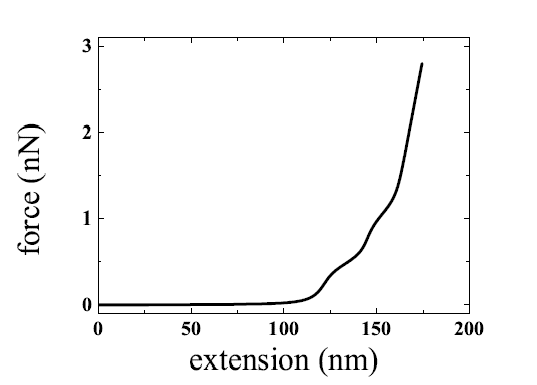
\includegraphics[width=0.7\textwidth,height=0.5\textwidth]{Figures/forceextension_CEWLC.png}%

\caption[Force extension curve: CEWLC]{Force-extension curve of a CEWLC model
that fits the experimental force-extension curve of a single polysaccharide
(pectin) chain\citep{schuster_hierarchical_2011} }
\label{fig:force_extension_CEWLC}
\end{center}
\end{figure}

\section{Networks of semiflexible chains:}
After the study of single chains, we have to study how all those chains interact
with themselves, with each other and with the media where they are.
The WLC is a model for ideal chains because the interaction between
monomers of the chain are ignored. This is not a problem in straight
(i.e. stiff) chains, but would be unreal in coiled chains, those are better
modeled with a self avoiding walk, where distant monomers cannot occupy the
same position, or with the inclusion of a excluded volume, that takes into
account the interaction between monomers, and the forbidden configurations.

The way the monomers of the chain interact with other monomers or with the
solvent has been studied for long time. The Flory interaction parameter $\chi$
which depends on temperature, and pressure of the system, is a way to
characterize it.
\begin{equation}\label{FloryInteraction}
\chi=\chi_{MS} - \frac{1}{2}(\chi_{MM} + \chi_{SS})
\end{equation}
where  $\chi_{MM}$ is related with monomer-monomer interactions. $\chi_{MS}$
with monomer-solvent, and $\chi_{SS}$ with solvent-solvent
interactions.

The relation between solvent, and monomers interaction can be classified using
$\chi$:
\begin{enumerate}
  \item Athermal. $\chi=0$. Solvent is very similar to ohter monomers. Simple
  examplest example of good solvent.
  \item Good solvent. $\chi<1/2$. Monomers of the chain prefer to interact with
  the solvent than with other monomers.
  \item Poor solvent. $\chi>1/2$. Monomers prefer to be closer to other
  monomers. For example, hydrophobic materials in water solvent.
  \item Theta solvent. $\chi=1/2$. Occurs at a temperature $T=\Theta$, and
  corresponds to the exact cancellation between steric repulsion and van der
  Waals attaction between monomers. The excluded volume:
  \begin{equation}\label{excludedvolume}
  \upsilon=(1-2\chi)a^3
  \end{equation}
  where $a$ is the effective length between monomers, is zero in theta solvents,
  and chains behaves as nearly ideal.\citep{gennes_scaling_1979}
\end{enumerate}

Also the concentration of polymers has important effects on the system. The
overlap threshold parameter $c*$ acts as an order parameter to distinguish dilute
polymer solutions, where the coils are separate, and more concentrated solution
where the chains overlap.
\begin{enumerate}
  \item Dilute. $c<c*$
  \item Dense. $c>c*$
  \item Semi-dilute. The chains do overlap but the polymer fraction
  $\phi=ca^3$ is still low $\phi*\ll\phi\ll1$. Since $\phi$ is small, the monomer-monomer interaction can
  be described very simple, such as the excluded volume parameter $\upsilon$ in
  \ref{excludedvolume}. In the case of dense systems we would need more complex
  relations used in liquids/fluids systems. 
\end{enumerate}


Gels: -> introduction of G

\section{Bulk Rheology}
\subsection{Linear viscoelasticity}
Any elastic material can be studied as a linear spring, whereby the
extension (strain) $\gamma$ is proportional to the applied stress $\sigma$ (force/area) :
$\sigma=G'\gamma$ , where G' is called the elastic modulus, and it is a measure
of sample's elasticity.

However the material response to the force, is not always that simple. Some
materials such as silk, rubber, and glass are subjected to a shear
stress and the corresponding Hooke's law deformation occurs, however it is
followed by a unexpected continious deformation termed as ``creep''. Upon
removal of the shear stress, certain materials come back to the initial state,
while other are permanently deformed. The phenomena of a time dependant shear
response is called viscolelasticity. \citep{macosko_rheology:_1994}.

To study the rheological (response of a material relating stress
and strain in fucntion of frequency) properties of a viscoelastic material, it
is applied an external sinusoidal strain, $\gamma(t)=\gamma_0\sin(\omega t)$. We
can expect (not always) that the stress output of the material will be:
$\sigma(t) = \sigma_0 \sin(\omega t + \delta)$. This stress output can be
analyzed by decomposition into two waves of frequency $\omega$, one in phase
with the strain, and the other $\pi/2$ out of phase:

\begin{equation}\label{viscoelastic-stress}
\sigma(t) = \sigma'(t) \sin(\omega t) + \sigma''(t)\cos(\omega t)
\end{equation}

where $ \tan \delta=\sigma''(t)/\sigma'(t)$. This allows the definition of two
moduli: $G'=\sigma'(t)/\gamma_0$ and $G''=\sigma''(t)/\gamma_0$ which are the
elastic (i.e. storage) modulus and viscous (i.e. loss) modulus respectively.

The stress can be expressed in terms of these two moduli:
\begin{equation}\label{viscoelastic-stress-G}
\sigma(t) = G'\gamma_0 \sin(\omega t) + G''\gamma_0\cos(\omega t)
\end{equation}

G'' has a physical meaning, it is associated with the energy dissipation per
cycle of deformation, which provides and indication of viscous loss
\citep{macosko_rheology:_1994}.
\subsection{Nonlinear behaviour: strain stiffening}

\begin{figure}[h]
\begin{center}
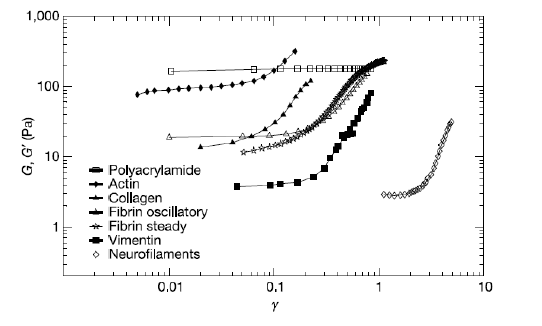
\includegraphics[width=0.7\textwidth,height=0.5\textwidth]{Figures/strainstiffening_storm.png}%

\caption[Strain-stiffening in semiflexible
polymers]{ Elastic shear moduli versus
strain. Strain-stiffening in a great range of different cross-linked biopolymer
networks\citep{storm_nonlinear_2005,carrillo_nonlinear_2013}}
\label{fig:strainstiffening-storm}
\end{center}
\end{figure}
 TODO
 Semiflexible networks:
Affine and non-affine deformations

Motivation of the topics selected:
Conclussion related with my role in the project. Bottom-up,networks,
entropic/enthalpic ways to describe strain-stiffening.

Ampliation of this topics will be done in function of future needs. A review of
the ignored dynamics of networks will be done for the final version of the
literature review.

END





%----------------------------------------------------------------------------------------
%	SECTION 2
%----------------------------------------------------------------------------------------

